\begin{center}
\underline{\large{Solución Ejercicio 3}} \\
\end{center}

Cálculo de Losas según Reglamentos 201/05 y 101/05. \\
\underline{Datos} \\
Exposición A1 $\Rightarrow$ H-20 \\
Acero ADN 42/50 \\
Recubrimiento Cc = 2cm

\begin{enumerate}
\item \underline{Predimensionado de losas en dos direcciones}

\begin{align*}
& h_{losa} = \frac{ln}{41} = \frac{(5.9m-0.2m)}{41} = 13.9cm \quad \text{De tabla 9.5.3.4}
\end{align*}
Adopto $h_{losa} = 15cm$

\begin{align*}
& b_W = 20cm \qquad b_W = 25cm\\
& h = 45cm \qquad h = 60cm
\end{align*}

Momento de inercia de la viga.

\begin{align*}
& I_{B1} = \frac{b \cdot h^3}{12} = \frac{25cm \cdot (60cm)^3}{12} = 450000cm^4\\
& I_{B2} = \frac{b \cdot h^3}{12} = \frac{20cm \cdot (45cm)^3}{12} = 151875cm^4
\end{align*}

Momento de inercia de la losa.

\begin{align*}
& I_{sy} = \frac{b \cdot h^3}{12} = \frac{440cm \cdot (15cm)^3}{12} = 123750cm^4\\
& I_{sx} = \frac{b \cdot h^3}{12} = \frac{590cm \cdot (15cm)^3}{12} = 165937cm^4\\
& \alpha_y = \frac{I_B}{I_{sy}} = \frac{450000cm^4}{123750cm^4} = 3.63 \\
& \alpha_x = \frac{I_B}{I_{sx}} = \frac{151875cm^4}{165937cm^4} = 0.915 \\
& \alpha_m = \frac{\alpha_x+\alpha_y}{2} = \frac{(3.63+0.915)}{2} = 2.27
\end{align*}

\newpage
Dado que $\alpha_m > 2 $ entonces:
\begin{align*}
& \alpha_m = 2.27 > 2 \\
& h \geq = \frac{l_w \cdot (0.80+ \frac{fy}{1400})}{36+ 9 \cdot \beta} \\
& h \geq = \frac{570cm \cdot (0.80+ \frac{420MPa}{1400})}{36+ 9 \cdot \frac{590cm}{440cm}} \\
& h \geq 13.05cm \\
& h_{min} \geq 9cm
\end{align*}

Adopto $h = 15cm$ \\
$h_{adoptado} = 15 cm \geq 13.05cm$ Verifica \\

\item \underline{Predimensionado de losas en una dirección}\\

\begin{itemize}
\item Losa L101
\begin{align*}
& h_{losa} = \frac{ln}{10} = \frac{110cm}{10} = 11cm \quad \text{De tabla 9.5.a}
\end{align*}
$h_{adoptado} = 15 cm \geq 11cm$ Verifica \\
\end{itemize}

\item \underline{Análisis de cargas}\\

\begin{itemize}
\item Losa L101: Uso Baño
\begin{align*}
& \text{Peso propio} \rightarrow 0.15m \cdot 2500 \frac{Kg}{m^3} = 375 \frac{Kg}{m^2} \Rightarrow 3.75 \frac{KN}{m^2} \\
& \text{Contrapiso} \rightarrow 0.07m \cdot 1600 \frac{Kg}{m^3} = 112 \frac{Kg}{m^2} \Rightarrow 1.12 \frac{KN}{m^2} \\
& \text{Cielorraso suspendido} \rightarrow  = 10 \frac{Kg}{m^2} \Rightarrow 0.10 \frac{KN}{m^2} \\
& \text{Piso + Carpeta} \rightarrow = 75 \frac{Kg}{m^2} \Rightarrow 0.75 \frac{KN}{m^2} \\
& D = 572 \frac{Kg}{m^2} \Rightarrow 5.72 \frac{KN}{m^2} \\
& L = 200 \frac{Kg}{m^2} \Rightarrow 2 \frac{KN}{m^2} \rightarrow \text{Según CIRSOC 101-05 - Capítulo 9}\\
& q_u = 1.2 \cdot D + 1.6 \cdot L = 1.2 \cdot 572 \frac{Kg}{m^2} + 1.6 \cdot 200 \frac{Kg}{m^2} = 1006.4 \frac{Kg}{m^2} \Rightarrow \framebox{$10.06 \frac{KN}{m^2}$} \\
& q_u = 1.4 \cdot D = 1.4 \cdot 572 \frac{Kg}{m^2} = 801 \frac{Kg}{m^2} \Rightarrow 8.1 \frac{KN}{m^2}
\end{align*}


\item Losa L102: Uso Cocina
\begin{align*}
& D = 572 \frac{Kg}{m^2} \Rightarrow 5.72 \frac{KN}{m^2} \\
& L = 200 \frac{Kg}{m^2} \Rightarrow 2 \frac{KN}{m^2} \rightarrow \text{Según CIRSOC 101-05 - Capítulo 9}\\
& Dpared = \frac{(0.2m \cdot 2.9m \cdot 2.70m \cdot 1600 \frac{Kg}{m^3}) \cdot 1.60}{2.90m \cdot 3.10m} = 446 \frac{Kg}{m^2} \\
& Dtotal = D + Dpared = 572 \frac{Kg}{m^2} + 446 \frac{Kg}{m^2} = 1018 \frac{Kg}{m^2} \\
& q_u = 1.2 \cdot D + 1.6 \cdot L = 1.2 \cdot 1018 \frac{Kg}{m^2} + 1.6 \cdot 200 \frac{Kg}{m^2} = 1541 \frac{Kg}{m^2} \Rightarrow \framebox{$15.41 \frac{KN}{m^2}$} \\
& q_u = 1.4 \cdot D = 1.4 \cdot 1018 \frac{Kg}{m^2} = 1425 \frac{Kg}{m^2} \Rightarrow 14.25 \frac{KN}{m^2}
\end{align*}

\item Losa L104: Uso Oficina
\begin{align*}
& D = 572 \frac{Kg}{m^2} \Rightarrow 5.72 \frac{KN}{m^2} \\
& L = 250 \frac{Kg}{m^2} \Rightarrow 2.5 \frac{KN}{m^2} \rightarrow \text{Según CIRSOC 101-05 - Capítulo 9}\\
& Dpared = \frac{(0.10m \cdot 2.7m \cdot 3.5m \cdot 1600 \frac{Kg}{m^3}) \cdot 1.50}{5.90m \cdot 4.40m} + \frac{(0.10m \cdot 2.7m \cdot 1m \cdot 1600 \frac{Kg}{m^3}) \cdot 1.70}{5.90m \cdot 4.40m}\\
& Dpared = 115.6 \frac{Kg}{m^2} \\
& Dtotal = D + Dpared = 572 \frac{Kg}{m^2} + 115.6 \frac{Kg}{m^2} = 688 \frac{Kg}{m^2} \\
& q_u = 1.2 \cdot D + 1.6 \cdot L = 1.2 \cdot 688 \frac{Kg}{m^2} + 1.6 \cdot 250 \frac{Kg}{m^2} = 1225 \frac{Kg}{m^2} \Rightarrow \framebox{$12.25 \frac{KN}{m^2}$} \\
& q_u = 1.4 \cdot D = 1.4 \cdot 688 \frac{Kg}{m^2} = 963 \frac{Kg}{m^2} \Rightarrow 9.63 \frac{KN}{m^2}
\end{align*}

\item Losa L105: Uso Comedor
\begin{align*}
& D = 572 \frac{Kg}{m^2} \Rightarrow 5.72 \frac{KN}{m^2} \\
& L = 200 \frac{Kg}{m^2} \Rightarrow 2 \frac{KN}{m^2} \rightarrow \text{Según CIRSOC 101-05 - Capítulo 9}\\
& q_u = 1.2 \cdot D + 1.6 \cdot L = 1.2 \cdot 572 \frac{Kg}{m^2} + 1.6 \cdot 200 \frac{Kg}{m^2} = 1006.4 \frac{Kg}{m^2} \Rightarrow \framebox{$10.06 \frac{KN}{m^2}$} \\
& q_u = 1.4 \cdot D = 1.4 \cdot 572 \frac{Kg}{m^2} = 801 \frac{Kg}{m^2} \Rightarrow 8.1 \frac{KN}{m^2}
\end{align*}

\item Losa L106: Uso Terraza
\begin{align*}
& D = 572 \frac{Kg}{m^2} \Rightarrow 5.72 \frac{KN}{m^2} \\
& L = 300 \frac{Kg}{m^2} \Rightarrow 3 \frac{KN}{m^2} \rightarrow \text{Según CIRSOC 101-05 - Capítulo 9}\\
& q_u = 1.2 \cdot D + 1.6 \cdot L = 1.2 \cdot 572 \frac{Kg}{m^2} + 1.6 \cdot 300 \frac{Kg}{m^2} = 1166 \frac{Kg}{m^2} \Rightarrow \framebox{$11.66 \frac{KN}{m^2}$} \\
& q_u = 1.4 \cdot D = 1.4 \cdot 572 \frac{Kg}{m^2} = 801 \frac{Kg}{m^2} \Rightarrow 8.1 \frac{KN}{m^2}
\end{align*}

\item Losa L107: Uso Terraza privada
\begin{align*}
& D = 572 \frac{Kg}{m^2} \Rightarrow 5.72 \frac{KN}{m^2} \\
& L = 300 \frac{Kg}{m^2} \Rightarrow 3 \frac{KN}{m^2} \rightarrow \text{Según CIRSOC 101-05 - Capítulo 9}\\
& q_u = 1.2 \cdot D + 1.6 \cdot L = 1.2 \cdot 572 \frac{Kg}{m^2} + 1.6 \cdot 300 \frac{Kg}{m^2} = 1166 \frac{Kg}{m^2} \Rightarrow \framebox{$11.66 \frac{KN}{m^2}$} \\
& q_u = 1.4 \cdot D = 1.4 \cdot 572 \frac{Kg}{m^2} = 801 \frac{Kg}{m^2} \Rightarrow 8.1 \frac{KN}{m^2}
\end{align*}

\end{itemize}


\item \underline{Momentos flectores}\\
\begin{itemize}
\item Losa L101

\begin{figure}[H]
\begin{center}
     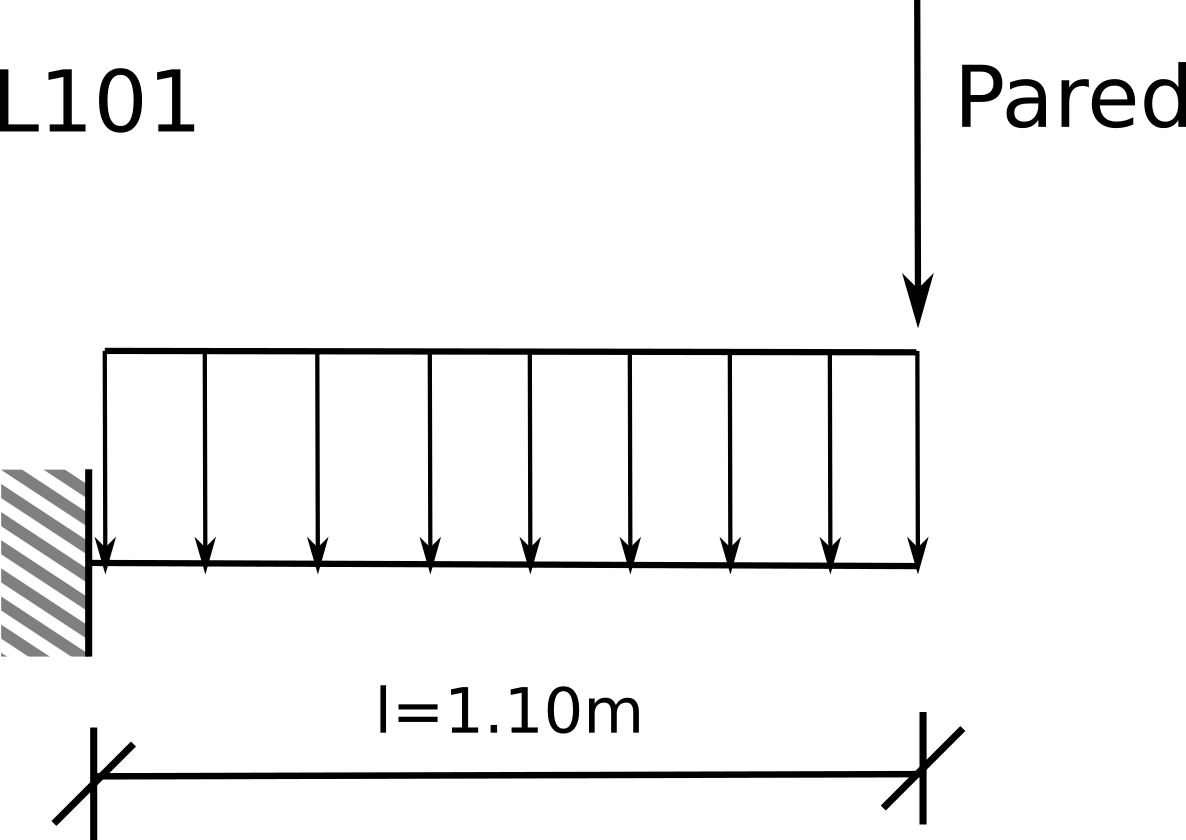
\includegraphics[scale = 1.3]{chapters/chapter_2/images/l101.png}
\end{center}
\end{figure}

\begin{align*}
& Mu_{xe} = \frac{U \cdot l^2}{2} +1.2 \cdot Dpared \cdot l \\
& Mu_{xe} = \frac{1 \frac{t}{m^2} \cdot (1.10m)^2}{2} + 1.2 \cdot (3m \cdot 1m \cdot 0.20m \cdot 1.6 \frac{t}{m^3}) \cdot 1.10m = 1.87 \frac{t \cdot m}{m}
\end{align*}

\newpage
\item Losa L102

\begin{figure}[H]
\begin{center}
     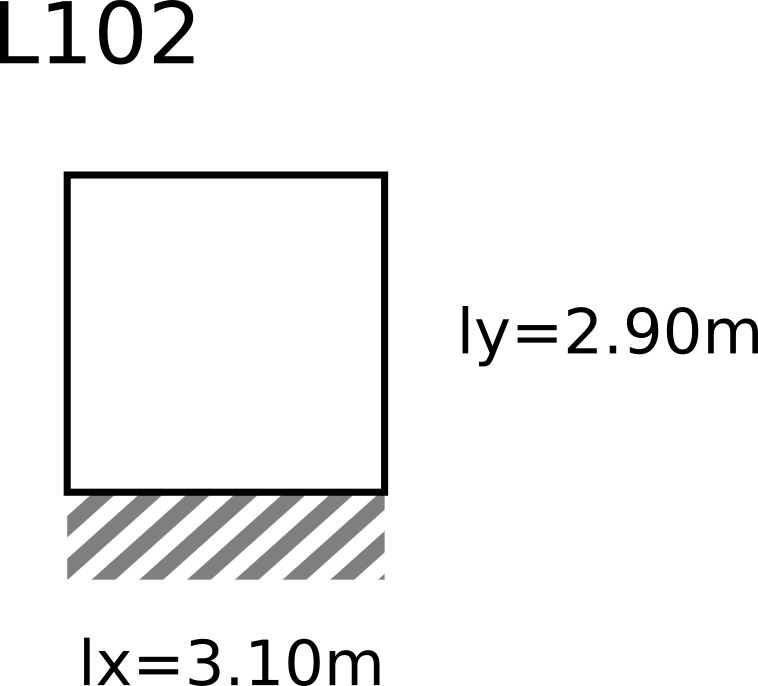
\includegraphics[scale = 1.3]{chapters/chapter_2/images/l102.png}
\end{center}
\end{figure}

\begin{align*}
& \frac{l_y}{l_x} = \frac{2.90m}{3.10m} = 0.95 \rightarrow \text{cambio de ejes} \quad \frac{l'_x}{l'_y} = 0.95\\
& m'_{xe} = 11.36 \rightarrow m_{ye} = 11.36 \\
& m'_x = 28.99 \rightarrow m_y = 28.99 \\
& m'_y= 42.74 \rightarrow m_x = 42.74 \\
& Mu_{ye} = \frac{U \cdot (lmenor)^2}{m_{ye}} = \frac{1.542 \frac{t}{m^2} \cdot (2.90m)^2}{11.36} = 1.14 \frac{t \cdot m}{m} \\
& Mu_y = \frac{U \cdot (lmenor)^2}{m_y} = \frac{1.542 \frac{t}{m^2} \cdot (2.90m)^2}{28.99} = 0.45 \frac{t \cdot m}{m} \\
& Mu_x = \frac{U \cdot (lmenor)^2}{m_x} = \frac{1.542 \frac{t}{m^2} \cdot (2.90m)^2}{42.74} = 0.30 \frac{t \cdot m}{m}
\end{align*}


\item Losa L104

\begin{figure}[H]
\begin{center}
     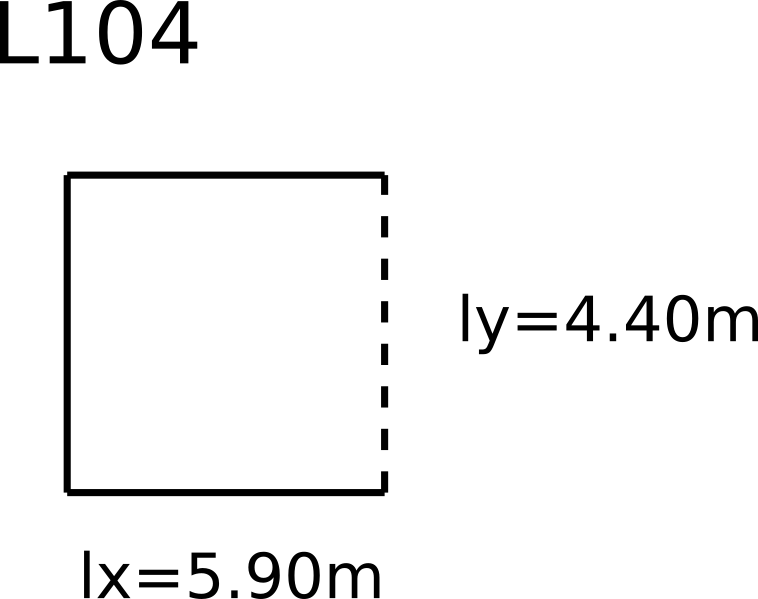
\includegraphics[scale = 1.3]{chapters/chapter_2/images/l104.png}
\end{center}
\end{figure}

\begin{align*}
& \frac{l'_y}{l'_x} = \frac{5.90m}{4.40m} = 1.34 \\
& m'_x = 11.09 \rightarrow m_y = 11.09 \\
& m'_y= 57.14 \rightarrow m_x = 57.14 \\
& Mu_y = \frac{U \cdot (lmenor)^2}{m_y} = \frac{1.225 \frac{t}{m^2} \cdot (4.40m)^2}{11.09} = 2.14 \frac{t \cdot m}{m} \\
& Mu_x = \frac{U \cdot (lmenor)^2}{m_x} = \frac{1.225 \frac{t}{m^2} \cdot (4.40m)^2}{57.14} = 0.42 \frac{t \cdot m}{m}
\end{align*}

\item Losa L105

\begin{figure}[H]
\begin{center}
     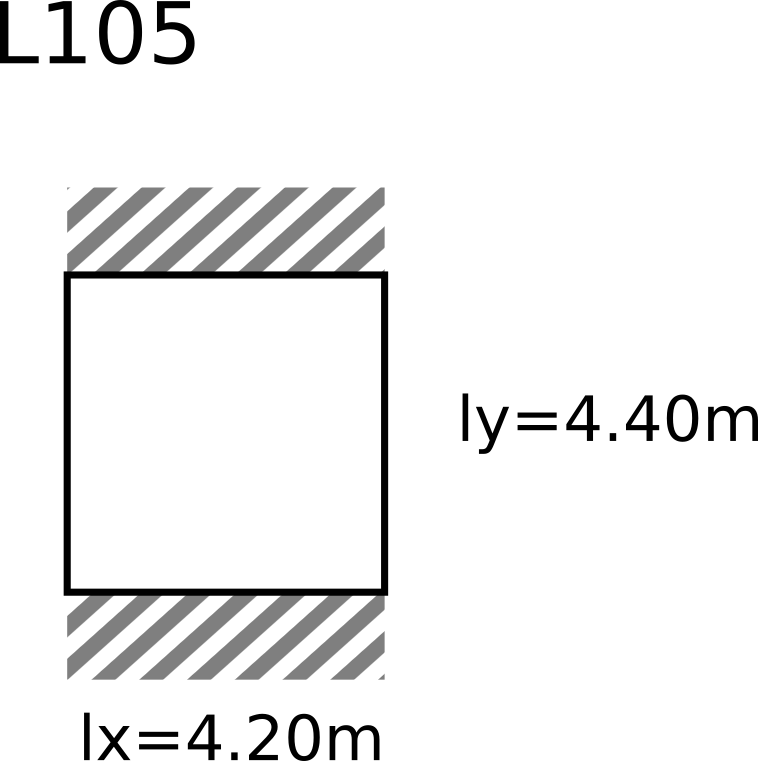
\includegraphics[scale = 1.3]{chapters/chapter_2/images/l105.png}
\end{center}
\end{figure}

\begin{align*}
& \frac{l_x}{l_y} = \frac{4.20m}{4.40m} = 0.95 \rightarrow \text{cambio de ejes} \quad \frac{l'_y}{l'_x} = 0.95\\
& m'_{xe} = 13.42 \rightarrow m_{ye} = 13.42 \\
& m'_x = 33.67 \rightarrow m_y = 33.67 \\
& m'_y= 52.91 \rightarrow m_x = 52.91 \\
& Mu_{ye} = \frac{U \cdot (lmenor)^2}{m_{ye}} = \frac{1.006 \frac{t}{m^2} \cdot (4.20m)^2}{13.42} = 1.32 \frac{t \cdot m}{m} \\
& Mu_y = \frac{U \cdot (lmenor)^2}{m_y} = \frac{1.006 \frac{t}{m^2} \cdot (4.20m)^2}{33.67} = 0.53 \frac{t \cdot m}{m} \\
& Mu_x = \frac{U \cdot (lmenor)^2}{m_x} = \frac{1.006 \frac{t}{m^2} \cdot (4.20m)^2}{52.91} = 0.34 \frac{t \cdot m}{m}
\end{align*}
\end{itemize}


\item \underline{Compatibilización de Momentos}\\

\begin{itemize}
\item Losas L102 y L105

\begin{align*}
& Mu_{ye} \quad 102-105 = \frac{1.32 \frac{t \cdot m}{m} + 1.14 \frac{t \cdot m}{m}}{2} = 1.23 \frac{t \cdot m}{m} \\
& Mu_y \quad 105 =  0.53 \frac{t \cdot m}{m} + (1.32 \frac{t \cdot m}{m} - 1.23 \frac{t \cdot m}{m})= 0.62 \frac{t \cdot m}{m}
\end{align*}

\end{itemize}

\newpage
\item \underline{Cálculo de Armaduras}\\
\begin{itemize}
\item Armadura Superior

\begin{align*}
& M_u = 1.87 \frac{t \cdot m}{m} \\
& M_n = \frac{M_u}{\phi} = \frac{1.87 \frac{t \cdot m}{m}}{0.9} = 2.08 \frac{t \cdot m}{m} \Rightarrow 0.0208 \frac{MN \cdot m}{m} \\
& d = h -db - Cc - \frac{db}{2} = 15cm - 1cm - 2cm - \frac{1cm}{2}= 11.5cm \\
& Kd = \frac{d}{\sqrt[]{\frac{M_n}{b}}} = \frac{0.115m}{\sqrt[]{\frac{0.0208 \frac{MN \cdot m}{m}}{1m}}} = 0.797 \Rightarrow Ke = 25.034 \\
& A_s = Ke \cdot \frac{M_n}{d} = 25.034 \cdot \frac{0.0208 \frac{MN \cdot m}{m}}{0.115m} = 4.53 \frac{cm^2}{m}\\
& As_{min} = 0.0018 \cdot b \cdot h = 0.0018 \cdot 100cm \cdot 15cm = 2.7 \frac{cm^2}{m}
\end{align*}

Se adopta A° superior $\phi$ 10 cada 15cm $\rightarrow \framebox{$5.24 \frac{cm^2}{m}$}$ \\

\underline{Verificación de separaciones}\\

\[ s = 15cm \leq \left\{ \begin{array}{ll}
         2.5 \cdot h = 2.5 \cdot 15cm = 37.5cm \quad \surd & \\
         25 \cdot db = 25 \cdot 1cm = 25cm \quad \surd &\\
         30cm \quad \surd & \end{array} \right. \] 
         
\[ s = 15cm \geq \left\{ \begin{array}{ll}
         db = 1cm \quad \surd & \\
         \geq 2.5cm \quad \surd &\\
         \geq \frac{4}{3} \cdot \text{Tamaño máximo del agregado} & \end{array} \right. \] 

\item Armadura Inferior

\begin{align*}
& M_u = 2.14 \frac{t \cdot m}{m} \\
& M_n = \frac{M_u}{\phi} = \frac{2.14 \frac{t \cdot m}{m}}{0.9} = 2.38 \frac{t \cdot m}{m} \Rightarrow 0.0238 \frac{MN \cdot m}{m} \\
& d = h -db - Cc - \frac{db}{2} = 15cm - 1cm - 2cm - \frac{1cm}{2}= 11.5cm \\
& Kd = \frac{d}{\sqrt[]{\frac{M_n}{b}}} = \frac{0.115m}{\sqrt[]{\frac{0.0238 \frac{MN \cdot m}{m}}{1m}}} = 0.745 \Rightarrow Ke = 25.207 \\
& A_s = Ke \cdot \frac{M_n}{d} = 25.207 \cdot \frac{0.0238 \frac{MN \cdot m}{m}}{0.115m} = 5.22 \frac{cm^2}{m}\\
& As_{min} = 0.0018 \cdot b \cdot h = 0.0018 \cdot 100cm \cdot 15cm = 2.7 \frac{cm^2}{m}
\end{align*}

Se adopta A° inferior $\phi$ 10 cada 15cm $\rightarrow \framebox{$5.24 \frac{cm^2}{m}$}$ \\

\underline{Verificación de separaciones}\\

\[ s = 15cm \leq \left\{ \begin{array}{ll}
         2.5 \cdot h = 2.5 \cdot 15cm = 37.5cm \quad \surd & \\
         25 \cdot db = 25 \cdot 1cm = 25cm \quad \surd &\\
         30cm \quad \surd & \end{array} \right. \] 
         
\[ s = 15cm \geq \left\{ \begin{array}{ll}
         db = 1cm \quad \surd & \\
         \geq 2.5cm \quad \surd &\\
         \geq \frac{4}{3} \cdot \text{Tamaño máximo del agregado} & \end{array} \right. \] 

\begin{align*}
& M_u = 0.62 \frac{t \cdot m}{m} \\
& M_n = \frac{M_u}{\phi} = \frac{0.62 \frac{t \cdot m}{m}}{0.9} = 0.69 \frac{t \cdot m}{m} \Rightarrow 0.0069 \frac{MN \cdot m}{m} \\
& d = h -db - Cc - \frac{db}{2} = 15cm - 1cm - 2cm - \frac{1cm}{2}= 11.5cm \\
& Kd = \frac{d}{\sqrt[]{\frac{M_n}{b}}} = \frac{0.115m}{\sqrt[]{\frac{0.0069 \frac{MN \cdot m}{m}}{1m}}} = 1.38 \Rightarrow Ke = 24.301 \\
& A_s = Ke \cdot \frac{M_n}{d} = 24.301 \cdot \frac{0.0069 \frac{MN \cdot m}{m}}{0.115m} = 1.46 \frac{cm^2}{m}\\
& As_{min} = 0.0018 \cdot b \cdot h = 0.0018 \cdot 100cm \cdot 15cm = 2.7 \frac{cm^2}{m}
\end{align*}

Se adopta A° inferior $\phi$ 8 cada 15cm $\rightarrow \framebox{$3.35 \frac{cm^2}{m}$}$ \\

\underline{Verificación de separaciones}\\

\[ s = 15cm \leq \left\{ \begin{array}{ll}
         2.5 \cdot h = 2.5 \cdot 15cm = 37.5cm \quad \surd & \\
         25 \cdot db = 25 \cdot 0.8cm = 20cm \quad \surd &\\
         30cm \quad \surd & \end{array} \right. \] 
         
\[ s = 15cm \geq \left\{ \begin{array}{ll}
         db = 0.8cm \quad \surd & \\
         \geq 2.5cm \quad \surd &\\
         \geq \frac{4}{3} \cdot \text{Tamaño máximo del agregado} & \end{array} \right. \] 

\end{itemize}
\end{enumerate}